\section{Versuchsdurchführung}

\subsection*{Kalibrierung des Aufbaus}

Vor Durchführung der Messungen wird durch Einstellung der Parameter der Elektronik das \emph{SQUID}-Signal
optimiert. Dazu wird dem Signal am Schwingkreis eine Dreiecksspannung überlagert,
so dass durch den dadurch verursachten Anstieg und Abfall des Magnetfelds am supraleitenden Ring
eine Flussänderung von mehr als einem Flussquant stattfindet. Dadurch wird ein Sinussignal vom \emph{SQUID}
generiert. Dieses Signal wird durch die Einstellung von Frequenz und Stromamplitude am Schwingkreis
maximiert und durch Anpassung des Offsets um den Nullpunkt zentriert.
\autoref{img:pattern} zeigt das gemessene Signal, dessen Amplitude maximiert wird.

%TODO Bild Pattern
\begin{figure}[H]
\begin{center}
  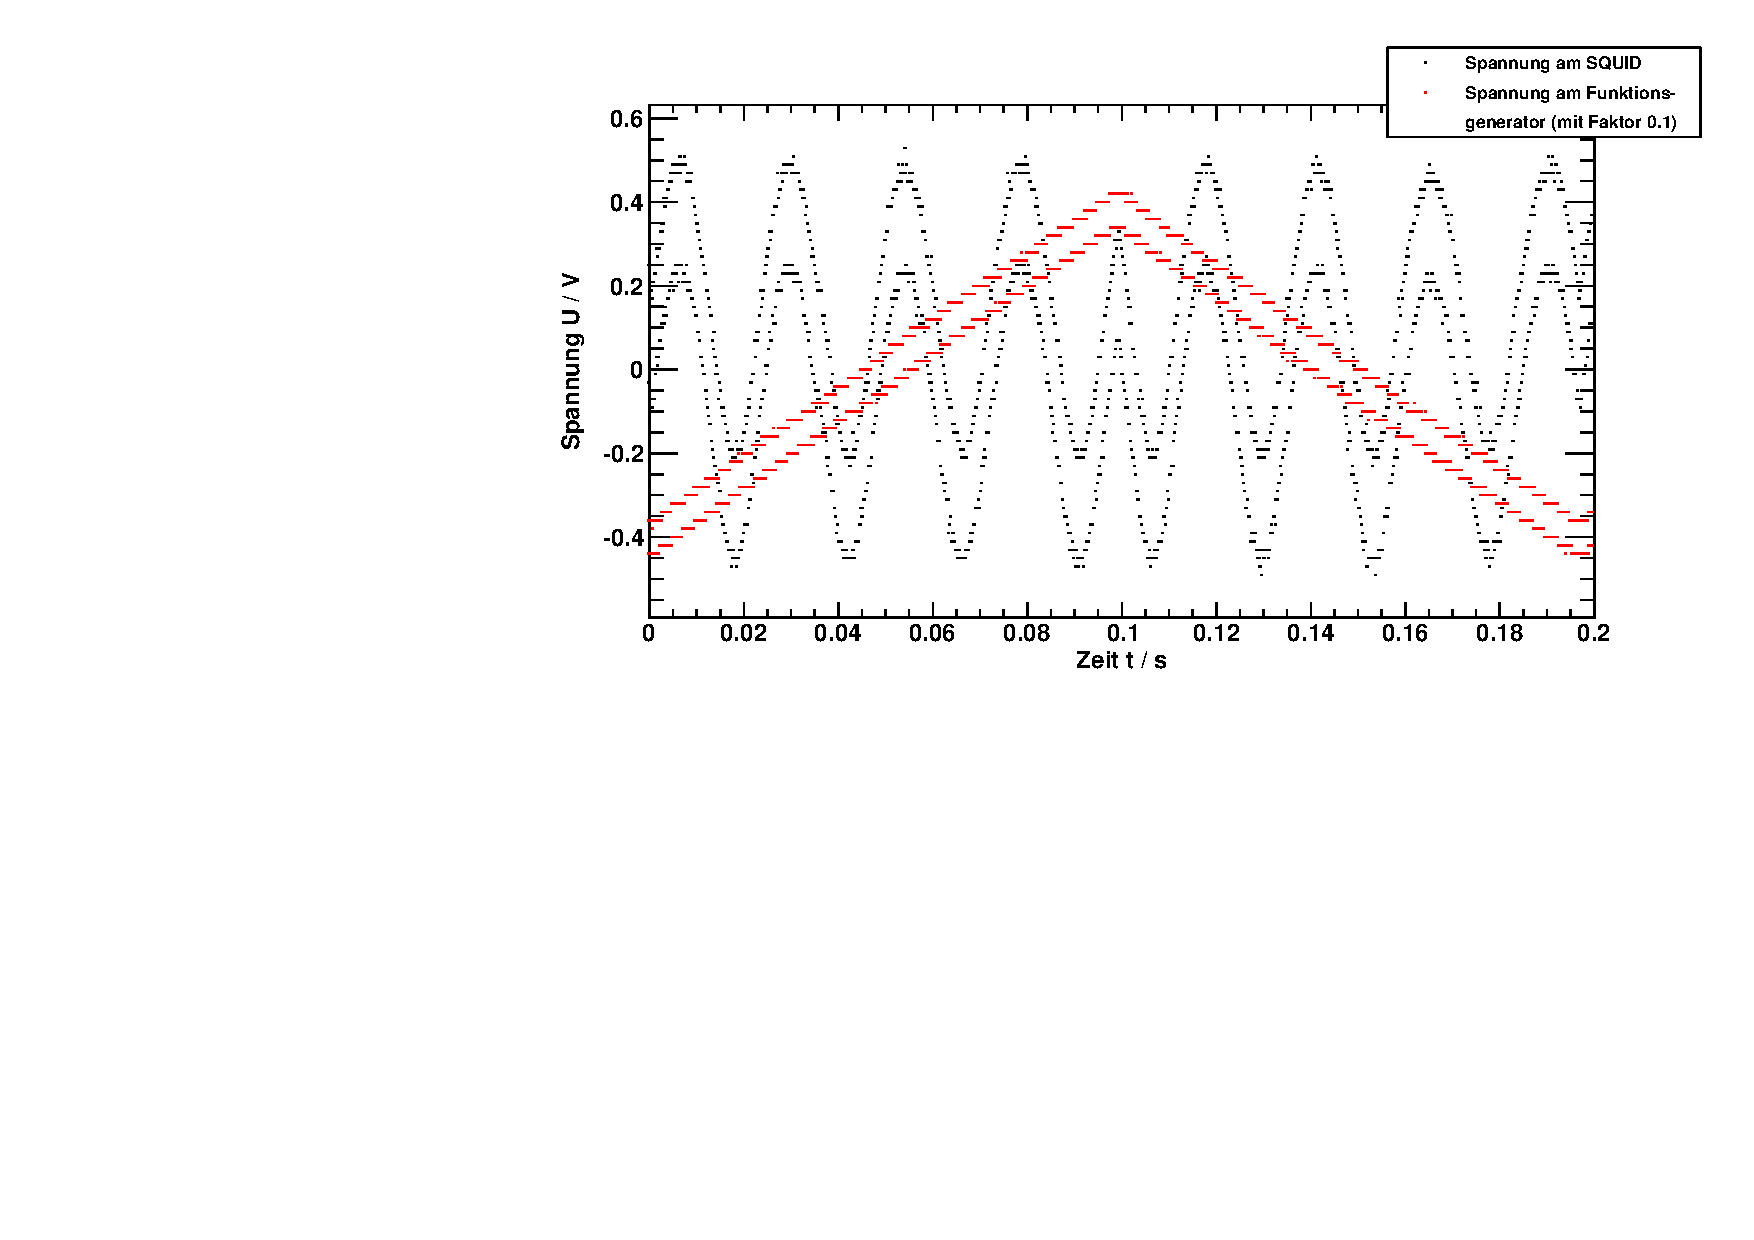
\includegraphics[width=\textwidth]{../img/pattern.pdf}
  \caption{Charakteristisches \emph{SQUID-pattern}, dessen Amplitude bei der Kalibrierung des Aufbaus
  maximiert wird. Die Ursache für die Aufspaltung der Signale in zwei Anteile ist nicht bekannt.}
  \label{img:pattern}
\end{center}
\end{figure}


\subsection*{Bestimmung des Magnetfelds verschiedener Proben}
Anschließend werden verschiedene Proben unter dem \emph{SQUID} eingebaut und von einem Motor
mit konstanter Geschwindigkeit gedreht.\\
An einer Leiterschleife werden fünf Messungen mit verschiedenen Strömen durchgeführt.
Außerdem werden ein Eisen-, ein Magnet- und ein Goldspan sowie ein Stabmagnet vermessen.
Zusätzlich wird eine Messung ohne Präparat sowie eine Messung mit leerem, rotierendem Probenhalter durchgeführt.



